\documentclass[a4paper, 11pt]{article}
\usepackage[left=2.5cm,right=2.5cm,top=3cm,bottom=3cm,a4paper]{geometry}
\usepackage{kotex}
\usepackage{color}
\usepackage{enumitem}
\usepackage{graphicx,subfigure}
\DeclareGraphicsExtensions{.pdf,.png,.jpg}




\title{\textbf{\Huge오목 한글 설명서}}
\author{\textbf{\LARGE5조}}
\begin{document}
   
   \maketitle
   
   \vspace{6cm}
\begin{center}
   \textbf{\large20134824김민석}\\
   \textbf{\large20134852허정건}\\
   \textbf{\large20134867이현문}\\
\end{center}
   
   
   
   
   \maketitle
   \newpage
   \thispagestyle{empty}        
   \mbox{}
   
   \begin{center} 
      \textbf{\Huge목차}\\
   \end{center}
   \vspace{1cm}
   \section{프로그램 채택 이유}
   \vspace{1cm}
   \section{프로그램 설명}
   \vspace{1cm}
   \section{사용 설명}
   \vspace{1cm}
   
   \section{기능 설명}
   \begin{enumerate}
      \item a설명
      \item b설명
      \item c설명

   
   \end{enumerate}

   

   
   \vspace{1cm}
   \section{버그와 개선할점}
   
   \vspace{1cm}
   \section{느낀점}
   
   
	\newpage
	\title{\textbf{\Huge1. 프로그램 채택 이유}}
	\\
   \ 다들 한번쯤 간단한 콘솔게임을 많이 해보셨을꺼라고 생각합니다. 그중 대표적인 게임으로 시작프로그램에 있는 윈도우즈용 간단한 게임들인 스파이더맨,지뢰찾기,프리쉘 등등 많이 있습니다. 하지만 최근 os가 윈도우10으로 바뀌면서 시작프로그램의 지뢰찾기등 많은 간단한 게임 프로그램들이 사라졌습니다. 저희는 이런 옛 추억적이고 학창시절 친구들과 자주했던 게임들중 여러개중 하나인 오목을 선택하게 되었습니다.
   
   
   
   \newpage
   \title{\textbf{\Huge2. 프로그램 설명}
   	\\ 이 콘솔프로그램은 네이버 어느유저가 올린 오픈소스프로그램으로써 간단한 오목을 즐기는 프로그램이다. 
   	
   	게임 방식 으론 키보드 방향키와 스페이스를 사용하여 가로, 세로 대각선으로 같은 색 알을 다섯 개 먼저 늘어놓으면 승리하는 게임으로, 상대방의 돌이 다섯 개가 되기 전에 라인 양 끝을 막여 것으로 방어한다. 
   
   
   
   \newpage
   \title{\textbf{\Huge5. 버그 }
   	
   \
  
   
   
   1. '룰'적용이 되지 않은 점
   : 프로그램 실행시작 화면에는 오목을 오랫동안 해왔던 사람도 몰랐던 
   룰이 '세 가지'가 있다라고 명확하게 표시가 되어있지만,
   정작 플레이를 하게 되면 그 룰을 적용하지 못하고
   세 가지 모드가 하나같이 똑같은 룰을 적용한다는 점을 알 수가 있다.
   
   (2). 게임 승리 혹은 패배 시, 실행 창 곧바로 종료
   : 일부 OS환경에서는 게임이 끝난 후, 메인화면으로 되돌아 가는 것이 아니라
   실행창이 종료되는 현상이 발견되었다.
   
   3. 육(6)목 이상 나열 했을 경우, 승리
   : 본 게임의 승리 규칙은 같은 색의 5개의 바둑돌이 나란히 나열되어 조건을 만족해야 한다.
   하지만, 본 프로그램은 5개를 초과한 6목 이상의 바둑돌이 나열되어 있는 경우도
   승리 조건에 포함시켜 규칙에 어긋난 경우이다.
   
   4. 기능이 동일한 U(Undo)와 R(Redo)
   : 둘 다 한 수 되돌리기의 기능으로 똑같은 기능을 다른 키로 구현한 점은 잘못되었다.
   
   \begin{figure}[h] %%% t: top, b: bottom, h: here
   	\begin{center}
   		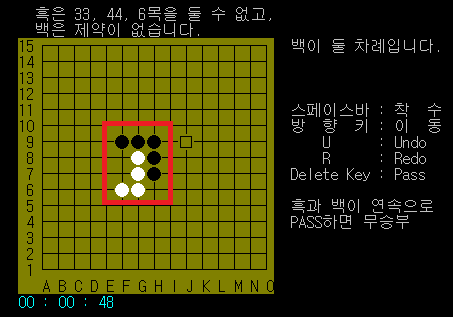
\includegraphics[width=0.7\linewidth]{OssOmok_2.png}
   	\end{center}
    \end{figure}
   
    
   \newpage
   \title{\textbf{\Huge6. 개선점 }
 
   	
   	\vspace{1cm}
   
   	
   	\begin{figure}[h] %%% t: top, b: bottom, h: here
   		\begin{center}
   			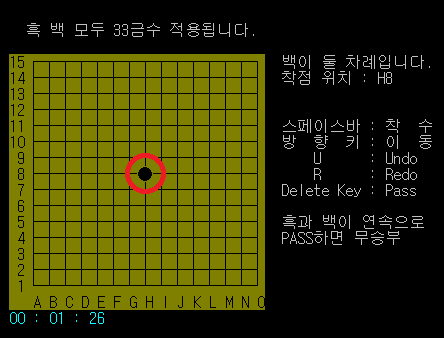
\includegraphics[width=0.7\linewidth]{OSS_1.png}
   		\end{center}
   	\end{figure}
   	
   	\ 1. 플레이어가 선흑일때, 흑백 아무제약이 없이 둘수있다고 조건문을 적어놨지만,
   	처음부터 흑,백이 하나씩 놓아져 있는 모습을 확인할 수 있었다.
   	-> 플레이어가 반드시 H8의 좌표값에서 시작하지 않을 수도 있음
   	
   	2. 결과 화면 승리자  '흑돌 승' 대신, 사용자 승리
   	
   	3. 전 화면으로 되돌리기
   	플레이 중에 ESC를 누르면 실행 첫 화면으로 되돌아 가지만,
   	첫 화면에서 룰을 선택 한 뒤의 화면에서는 ESC를 눌러도 첫 화면으로 되돌아가지 않았다.
   	
   	4. 버튼 기능중에 'Delete Key'의 Pass가 뭔지 궁금하지 않던가?
   	차라리 '='의 버튼을 눌러 Draw로 표시하는 것이 사용자를 위한 배려가 돋보이지 않나 싶다.
   	
   	5. 제한시간을 두어 긴장감 있는 게임을 조성하면 좋을 것 같다.
   	

    
\end{document} 